% !TEX TS-program = pdflatex
% !TEX encoding = UTF-8 Unicode

% This file is a template using the "beamer" package to create slides for a talk or presentation
% - Giving a talk on some subject.
% - The talk is between 15min and 45min long.
% - Style is ornate.

% MODIFIED by Jonathan Kew, 2008-07-06
% The header comments and encoding in this file were modified for inclusion with TeXworks.
% The content is otherwise unchanged from the original distributed with the beamer package.

\documentclass[handout]{beamer}


% Copyright 2004 by Till Tantau <tantau@users.sourceforge.net>.
%
% In principle, this file can be redistributed and/or modified under
% the terms of the GNU Public License, version 2.
%
% However, this file is supposed to be a template to be modified
% for your own needs. For this reason, if you use this file as a
% template and not specifically distribute it as part of a another
% package/program, I grant the extra permission to freely copy and
% modify this file as you see fit and even to delete this copyright
% notice. 


\mode<presentation>
{
  %\usetheme{Rochester}
  %\usetheme{Marburg}
  %\usetheme{Madrid}
  %\usetheme{Luebeck}
  \usetheme{Frankfurt}
  %\usetheme{Dresden}
  %\usetheme{Copenhagen}
  %\usetheme{Berlin}
  %\usetheme{Warsaw}

  %\setbeamercovered{transparent}
  % or whatever (possibly just delete it)

	\setbeamertemplate{navigation symbols}{}%remove navigation symbols
}


\usepackage[ngerman]{babel}
% or whatever

\usepackage[utf8x]{inputenc}
% or whatever

%\usepackage{times}
\usepackage{lmodern}
\usepackage[T1]{fontenc}
% Or whatever. Note that the encoding and the font should match. If T1
% does not look nice, try deleting the line with the fontenc.


\title[COBOL-\"Uberblick]   % (optional, use only with long paper titles)
{COBOL}

\subtitle
{Die erste Programmiersprache für Wirtschaftsanwendungen} % (optional)

\author % (optional, use only with lots of authors)
{Sebastian Deußer}
% - Use the \inst{?} command only if the authors have different
%   affiliation.

%\institute[Universities of Somewhere and Elsewhere] % (optional, but mostly needed)
%{
%  \inst{1}%
%  Department of Computer Science\\
%  University of Somewhere
%  \and
%  \inst{2}%
%  Department of Theoretical Philosophy\\
%  University of Elsewhere}
% - Use the \inst command only if there are several affiliations.
% - Keep it simple, no one is interested in your street address.

%\date[Short Occasion] % (optional)
%{Date / Occasion}

%\subject{COBOL \"Ubersicht}
% This is only inserted into the PDF information catalog. Can be left
% out. 



% If you have a file called "university-logo-filename.xxx", where xxx
% is a graphic format that can be processed by latex or pdflatex,
% resp., then you can add a logo as follows:

% \pgfdeclareimage[height=0.5cm]{university-logo}{university-logo-filename}
% \logo{\pgfuseimage{university-logo}}



% Delete this, if you do not want the table of contents to pop up at
% the beginning of each subsection:



% If you wish to uncover everything in a step-wise fashion, uncomment
% the following command: 

%\beamerdefaultoverlayspecification{<+->}


\begin{document}

\begin{frame}
  \titlepage
\end{frame}

%\begin{frame}{Namensbedeutung}
  % You might wish to add the option [pausesections]
%\end{frame}


% Since this a solution template for a generic talk, very little can
% be said about how it should be structured. However, the talk length
% of between 15min and 45min and the theme suggest that you stick to
% the following rules:  

% - Exactly two or three sections (other than the summary).
% - At *most* three subsections per section.
% - Talk about 30s to 2min per frame. So there should be between about
%   15 and 30 frames, all told.

\section{Übersicht}

\subsection{Namensbedeutung}

\begin{frame}{Namensbedeutung}
	\begin{itemize}
		\item
			COBOL steht für COmmon Business-Oriented Language.
		\item
			entwickelt für betriebswirtschaftliche Programme (im Gegensatz zum technische-wissenschaftliche Anwendungen Fokus anderer Sprachen).
	\end{itemize}
\end{frame}

\subsection{Historische Entwicklung}

\begin{frame}{Anfänge}
	\begin{itemize}
		\item
			entwickelt durch Arbeitsgruppe in der 2. H\"alfte von 1959
		\item
			federführend war Grace Hopper, die Erfinderin des ersten Compilers (A-0) und Mitentwicklerin einiger fr\"uher Computer (zB Harvard Mark I+II, UNIVAC I)
		\item
			basierte auf Hoppers FLOW-MATIC und IBMs COMTRAN (``Business-Version'' von FORTRAN)
		\item
		offizielle Festlegung des Standards (COBOL 60) am 03. Januar 1960, danach individuelle (inkompatibele) Erweiterungen von verschiedenen Firmen
	\end{itemize}
\end{frame}

\begin{frame}{Versionen des Standards}
	\begin{itemize}
		\item
			ANS COBOL 1968: ANSI Standard um die verschiedenen \"Anderungen nach 1959 zu einer kompatiblen Basis zusammenzufassen
		\item
			COBOL 1974: 2. ANSI Standard, neue Features ein wie Datei-Organisation, Report Modul, Segmentierungsmodul; Abschaffung von Features ab wie das \texttt{NOTE} Statement, inkompatibel zu vorherigen Standards
		\item
			COBOL 1985: \"uberarbeiteter ANSI Standard, Einf\"uhrung G\"ultigkeitsbereich-Terminatoren wie \texttt{END-IF}, Features wie geschachtelte Unterprogramme, die Statements \texttt{CONTINUE}, \texttt{EVALUATE}, \texttt{INITIALIZE}, die Operatoren >= und <=, Referenz Modifikation
	\end{itemize}
\end{frame}

\begin{frame}{Entwicklung um und nach 2000}
		\begin{itemize}
			\item
				viele in den 80ern und davor geschriebenen Programme verwendeten Records mit Datumsfeldern mit fester 2 stelliger Jahreszahl
			\item
				=> um 1999/2000 rum Massensterben unter COBOL Anwendungen wegen Y2K-Bug; Programme mussten entweder grundlegend überarbeitet oder ganz ersetzt werden 
			\item
				COBOL 2002 und objekorientiertes COBOL: Anfang der 90er wurde entschieden das dem n\"achste Standard von COBOL Objektorientierung hinzugef\"ugt werden sollte
		\end{itemize}
\end{frame}

\section{Einsatz}

\subsection{Einsatzgebiete}

\begin{frame}{Einsatzgebiete}
	\begin{itemize}
		\item
			Haupteinsatzgebiet ist betriebswirtschaftliche Datenverarbeitung
		\item
			bei klassischer Aufteilung nach Benutzerschnittstelle, Verabreitungsteil und Datenhaltungsteil stellt COBOL normal den Verarbeitungsteil eine EDV-Programms
	\end{itemize}
\end{frame}

\subsection{heutiger Einsatz}

\begin{frame}{heutiger Einsatz}
	\begin{itemize}
		\item
			COBOL hatte wenig Einfluss auf sp\"atere Programmiersprachen da Fokus auf relativ simple Algorithmen und hohes I/O-Volumen akademisch uninteressant
		\item
			die meisten noch verwendeten COBOL Anwendungen sind Teil von jahrzehntelang gewachsene Systeme, komplette Neuentwicklungen finden nur noch selten in COBOL statt
		\item
			2009 wurden geschätzt \"uber 40 Milliarden Zeilen COBOL Code in Industrieprogrammen verwendet, Wachstumsrate 4 Milliarden Zeilen Code pro Jahr
		\item
			SAPs Programmiersprache ABAP wurde sehr stark von COBOL beeinflusst
	\end{itemize}
\end{frame}

\section{Vor- und Nachteile}

\subsection{Vorteile}

\begin{frame}{Vorteile}
	\begin{itemize}
		\item
			entworfen um Programme auf verschiedener Hardware laufen zu lassen ohne große Ver\"anderung des Codes
		\item
			durch mehrstufiges Design der einzelnen Programmsprachen-Module lassen sich COBOL-Programme auf sehr eingeschr\"ankter Hardware mit geringen Anpassungen ausf\"uhren
		\item
			der ANSI-Standard wird durchschnittlich alle 10-15 Jahre an neue Gegebenheiten angepasst, z.B. kam 2002 Unterstüzung für Objektorientierung dazu
		\item
			es gibt einen kostenlosen quelloffenen Compiler namens GNU COBOL (ehemals OpenCOBOL) für POSIX-kompatible Betriebssysteme
	\end{itemize}
\end{frame}

\subsection{Nachteile}

\begin{frame}{Nachteile}
	\begin{itemize}
		\item
		    bis COBOL 74 gab es keine M\"oglichkeit Programme zu strukturieren, zB waren alle Variablen global
		\item
			aufgrund vieler Eigenentwicklungen von Firmen und anderen Gruppen gibt es viele verschiedene Standards von COBOL die teilweise inkompatibel zueinander sind
		\item
			da die Syntax sich an geschriebenem Englisch orientiert werden COBOL Programme schnell recht langwierig zu schreiben
	\end{itemize}
\end{frame}

\section{Praxis}

\subsection{Entwicklungsumgebung}

\begin{frame}{Entwicklungsumgebung}
	\begin{itemize}
		\item
			viele Computer/Betriebsystemhersteller (zB IBM, Siemens, Unisys, HP) entwickelten (und vertreiben teilweise auch heute noch) eigene Compiler, teilweise mit eigenen Erweiterungen des Standards
		\item
			es gibt verschiedene Codegeneratoren die COBOL-Programme oder Teile davon generieren um die Entwicklungsarbeit zu erleichtern
		\item
			Plugins für viele gängige IDEs, z.B. cobolclipse für Eclipse
	\end{itemize}
\end{frame}

\begin{frame}{Entwicklungsumgebung (2)}
	\begin{itemize}			
		\item
			verbreiteste (kommerzielle) COBOL IDE ist Visual COBOL von Micro Focus; besitzt moderne Features wie Generierung von Java Byte-Code, .NET Unterstützung und Webservices
		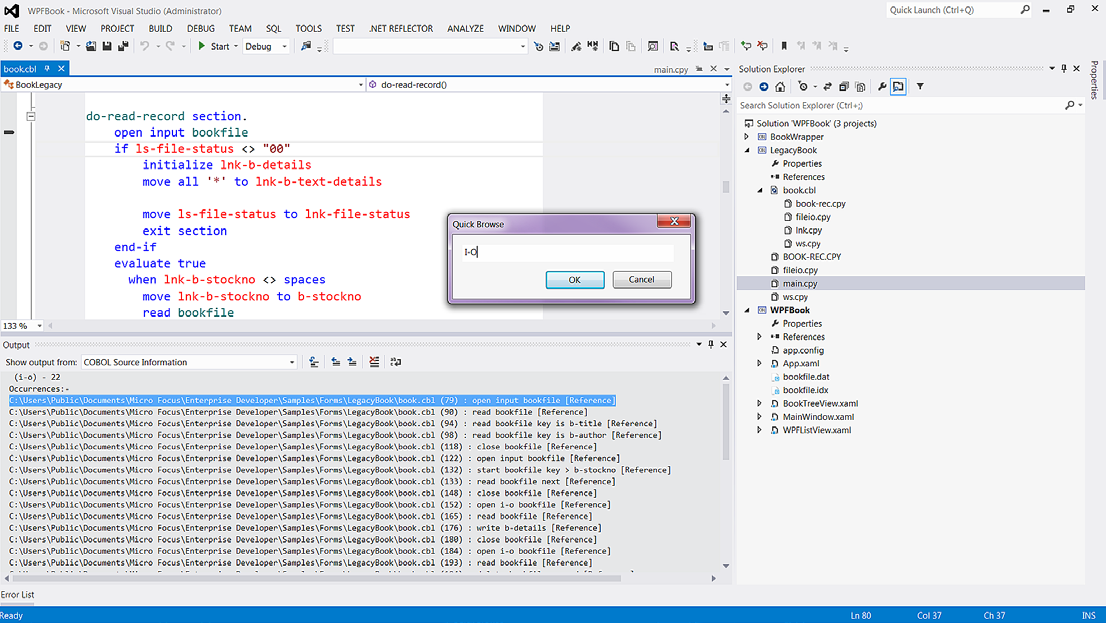
\includegraphics[width=9cm]{VisualCOBOL2}
	\end{itemize}
\end{frame}

\subsection{Sprachspezifikation}

\begin{frame}{Sprachspezifikation}
	\begin{itemize}
		\item
			COBOL wurde so entworfen das der Code relativ lesbarem Englisch entspricht (z.B. \texttt{ADD b TO c GIVING a} f\"ur a = b + c)
		\item
			importieren von Programmteilen als sgn. Copybooks mit dem Befehl \texttt{COPY}, vergleichbar mit \texttt{\#include} in C u.\"A.
		\item
			Standard Kontrollstrukturen wie 
	\end{itemize}
\end{frame}

\begin{frame}{Datenstrukturen}
	\begin{itemize}
		\item
			Grunddatenstruktur ist ein sogenannter Record, ein multidimensionales heterogenes Array
		\item
			Records k\"onnen mit gew\"ohnlicheren homogenen Arrays gemischt verwendet werden, ein Array kann also Inhalt eines Records sein und umgekehrt
		\item
			über die \texttt{PICTURE} Klausel kann man den Inhalt (inklusive Feldgrößen) von Records exakt definieren
		\item
			Variablen müssen bei der Deklaration typisiert werden, allerdings hat man Dank Records und der \texttt{PICTURE} Klausel vergleichsweise viel Freiheit dabei
	\end{itemize}
\end{frame}

\begin{frame}{Aufteilung eines Programms}
	\begin{itemize}
		\item
			jedes Programm besteht aus 4 Teilen zum trennen von:
			\begin{itemize}
			 \item hardwareabh\"angigem und unabh\"angigem Code
			 \item Algorithmen Beschreibungen und Daten Beschreibungen
			 \end{itemize}
		\item
			\texttt{IDENTIFICATION}: beginnt jedes Programm, benennt Programm und den Autor (Autor optional), für andere Kommentare als Dokumentation
		\item
			\texttt{ENVIRONMENT}: beinhaltet maschinenabhängige Programmspezifikationen wie zB Verbindungen zwischen dem Programm und externen Daten
		\item
			\texttt{PROCEDURE}: beinhaltet die Algorithmen
		\item
			\texttt{DATA}: beinhaltet die Daten Beschreibungen
	\end{itemize}
\end{frame}

\begin{frame}{Sequenzkontrolle}
	\begin{itemize}
		\item
			
	\end{itemize}
\end{frame}

\begin{frame}{Quellen}
	\begin{itemize}
		\item
			\url{http://en.wikipedia.org/wiki/COBOL}
		\item
			\url{http://de.wikipedia.org/wiki/COBOL}
		\item
			Terrence W. Pratt - Programming Languages: Design and Implementation (Prentice Hill 1975)
		\item OpenCOBOL Programmers Guide
	\end{itemize}
\end{frame}

%\begin{frame}{Make Titles Informative.}
%
%  You can create overlays\dots
%  \begin{itemize}
%  \item using the \texttt{pause} command:
%    \begin{itemize}
%    \item
%      First item.
%      \pause
%    \item    
%      Second item.
%    \end{itemize}
%  \item
%    using overlay specifications:
%    \begin{itemize}
%    \item<3->
%      First item.
%    \item<4->
%      Second item.
%    \end{itemize}
%  \item
%    using the general \texttt{uncover} command:
%    \begin{itemize}
%      \uncover<5->{\item
%        First item.}
%      \uncover<6->{\item
%        Second item.}
%    \end{itemize}
%  \end{itemize}
%\end{frame}
%
%
%
%
%\section*{Summary}
%
%\begin{frame}{Summary}
%
%  % Keep the summary *very short*.
%  \begin{itemize}
%  \item
%    The \alert{first main message} of your talk in one or two lines.
%  \item
%    The \alert{second main message} of your talk in one or two lines.
%  \item
%    Perhaps a \alert{third message}, but not more than that.
%  \end{itemize}
%  
%  % The following outlook is optional.
%  \vskip0pt plus.5fill
%  \begin{itemize}
%  \item
%    Outlook
%    \begin{itemize}
%    \item
%      Something you haven't solved.
%    \item
%      Something else you haven't solved.
%    \end{itemize}
%  \end{itemize}
%\end{frame}


\end{document}


